\chapter{Reinforcement learning in dialogue processing}
\label{ch:soarl}

\section{Reinforcement Learning}
\label{soa:rl}

	\subsection{Reinforcement in biology}
    
		Reinforcement Learning (RL) is a sub-field of machine learning where an agent is put into an environment to interact with, and figures out through the process of \textit{trial and error} what the best actions to take are, given a reward function to maximise \cite{Sutton1998} (see Figure \ref{fig:rlscheme}\footnote{This figure is taken from \cite{Sutton1998}.}).
			
			\begin{figure*}[ht]
				\centering
				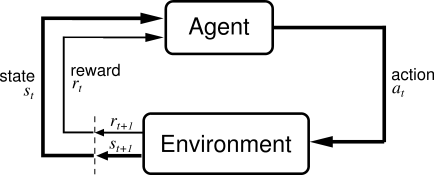
\includegraphics[scale=0.7]{figures/rl.png}
				\caption{The interaction cycle between the agent and the environment in reinforcement learning}
				\label{fig:rlscheme}
			\end{figure*}
			
			It was first inspired by the field of biology where living organisms are considered as the agents. Rewards are associated with stimuli that the agent seeks like food for example. Conversely, punishments are stimuli that it tries to avoid like important heat for instance. In \cite{Thorndike1898}, hungry animals where put in enclosures where the only way to escape and find food is to perform some simple act (pulling at a loop of cord, pressing a lever, stepping on a platform...). If after a certain period of time they were not able to escape, they are taken out of the box without being immediately fed. This experiment showed how animals were able to learn what to do in order to escape from the enclosure.
			
			During the last two decades, similarities between reinforcement learning and neurons behaviours in the brain were also discovered. In \cite{Schultz1995,Schultz1998}, similarly to the previous experiment, monkeys were put in situations where the accomplishment of an action is necessary to get food. Then the reaction of their dopamine neurons was analysed. Among many other applications where reinforcement learning meets neuroscience, \cite{Doya2007} commented on this experiment: \textit{Although dopamine neurons initially responded to the rewards, when those rewards became fully predictable from preceding sensory cues, such as light and sound, their reward responses went away. Instead, dopamine neurons started to respond to reward-predictive sensory cues. If the reward is omitted after learning, dopamine neuron firing was suppressed at the timing when reward delivery is expected. These are interesting findings on their own, but most exciting for those who are familiar with reinforcement learning theory because it exactly matches what the TD error does}.
			
		\subsection{Markov Decision Processes}
        
			The most common model consists in casting the problem as a Markov Decision Process (MDP) which is a quintuple $\mathcal{M} = (\mathcal{S},\mathcal{A},\mathscr{T},\mathscr{R},\gamma)$ where:
			\begin{itemize}
					\item $\mathcal{S}$ is the \textit{state space}. At each time step $t$, the agent is in some state $s_t \in \mathcal{S}$.
					\item $\mathcal{A}$ is the \textit{action space}. At each time step $t$, the agent decides to take action $a_t \in \mathcal{A}$.
					\item $\mathscr{T}$ is the \textit{transition model} where each $(s,a,s')$ in $\mathcal{S} \text{x} \mathcal{A} \text{x} \mathcal{S}$ is associated with a real number in $[0,1]$ corresponding to the probability $\mathbb{P} (s_{t+1} = s'|s_t = s, a_t=a)$. A more compact notation will be used in the following: $\mathscr{T}_{ss'}^a = \mathscr{T} (s,a,s')$.
					\item $\mathscr{R}$ is the \textit{reward model}. Let $r$ be the immediate reward due to taking action $a$ in state $s$, then $\mathscr{R}$ is the set of distributions of $r$ for every $(s,a) \in \mathcal{S} \text{x} \mathcal{A}$. The following notation will be used in the rest of this chapter: $\mathscr{R}_{ss'}^a = \mathbb{E} [\mathscr{R} (s,a,s')|s,a,s']$.
					\item $\gamma \in [0,1)$ is referred to as the \textit{discount factor}. In the RL framework, the aim of the agent is not to maximise the immediate reward but the \textit{expected return}, where the return $R_t$ is defined as follows:
					
					\begin{eqnarray}
						R_t & = & r_{t+1} + \gamma r_{t+2} + \gamma^2 r_{t+3} + ... \nonumber \\
						& = & \sum_{k=0}^\infty \gamma^k r_{t+k+1} \label{eq:return}
					\end{eqnarray}
					
					Therefore, when $\gamma = 0$, the agent maximises the immediate reward only and when $\gamma$ tends towards 1, the agent maximises the sum of all the future rewards. In other words, the parameter $\gamma$ controls how far-sighted is the agent in terms of future rewards.
	\end{itemize}
			
			A \textit{policy} $\pi : \mathcal{S} \rightarrow \mathcal{A}$ is a mapping between the state space and the action space. An agent is said to follow the policy $\pi$ when for each time $t$, it takes the action $a_t = \pi(s_t)$. A policy can also be stochastic, in which case, $\pi (s,a)$ denotes the probability of choosing action a when the agent is in state s. A key aspect of MDPs is the \textit{Markov property}. Being in state $s$ is the only information available to predict the future, and adding information about what happened during previous time steps has no power of prediction. Therefore, given a policy, each state $s \in \mathcal{S}$ is associated with a value $V^\pi (s)$ which is the expected return when in this state and following the policy $\pi$ afterwards:
				
				\begin{eqnarray}
					V^{\pi} (s_t) & = & \mathbb{E} [R_t | s_t, \pi] \label{eq:valuefunc}
				\end{eqnarray}
					
			Another interesting quantity is the expected return knowing the current state but also the next action, after which $\pi$ is followed. This is referred to as the Q-function:
				
				\begin{eqnarray}
					Q^{\pi} (s_t,a_t) & = & \mathbb{E} [R_t | s_t, a_t, \pi] \label{eq:qfunc}
				\end{eqnarray}
					
			Given the definition of $R_t$, one can notice that 
			\begin{eqnarray}
					V^{\pi} (s_t)   & = & \mathbb{E} [R_t | s_t, \pi] \nonumber \\
					& = & \mathbb{E} [r_t + \gamma \sum_{k=0}^\infty \gamma^k r_{(t+1)+k+1} | s_t, \pi] \nonumber \\
					& = & \mathbb{E} [r_t + \gamma R_{t+1} | s_t, \pi] \nonumber \\
					& = & \mathbb{E} [r_t + \gamma \mathbb{E} [R_{t+1}|s_{t+1}, \pi] | s_t, \pi] \nonumber \\
					& = & \mathbb{E} [r_t + \gamma V^{\pi} (s_{t+1}) | s_t, \pi] \label{eq:vbellman}
			\end{eqnarray}
					
		This is known as the Bellman equation for $V^{\pi}$ and it can also be written for the Q-function, as follows
				
				\begin{eqnarray}
					Q^{\pi} (s_t,a_t) & = & \mathbb{E} [r_t + \gamma Q^{\pi} (s_{t+1}, \pi(s_{t+1})) | s_t, a_t, \pi] \label{eq:qbellman}
				\end{eqnarray}
	
	\subsection{Reinforcement Learning}
            
			A natural question that can be asked at this point is: how are these values computed? In reinforcement learning, this is known as the \textit{evaluation problem}. The transition model $\mathscr{T}$ and the reward model $\mathscr{R}$ are the elements that define the dynamics of the MDP. If they are known, $V^{\pi}$ can be directly computed:
			
			\begin{eqnarray}
					V^{\pi} (s)   & = & \mathbb{E} [R_t | s_t = s, \pi] \nonumber \\
					& = & \sum_{a \in \mathcal{A}} \pi (s,a) \mathbb{E} [R_t | s_t = s, a_t = a, \pi] \nonumber \\
					& = & \sum_{a \in \mathcal{A}} \pi (s,a) \mathbb{E} [r_t + \gamma R_{t+1} | s_t = s, a_t = a, \pi] \nonumber \\
					& = & \sum_{a \in \mathcal{A}} \pi (s,a)  \sum_{s' \in \mathcal{S}} \mathscr{T}_{ss'}^a (\mathscr{R}_{ss'}^a + \gamma \mathbb{E} [R_{t+1} | s_{t+1} = s', \pi]) \nonumber \\
					& = & \sum_{a \in \mathcal{A}} \pi (s,a)  \sum_{s' \in \mathcal{S}} \mathscr{T}_{ss'}^a (\mathscr{R}_{ss'}^a + \gamma V^{\pi} (s')) \label{eq:dynprog}
			\end{eqnarray}
					
			It is possible to define an order over the policies. Saying that $\pi_1$ is better that $\pi_2$ means that for all the states $s$, $V^{\pi_1} (s) \geq V^{\pi_2} (s)$. It can be shown that there exists at least one policy that is better than all the others: it is called the \textit{optimal policy} ($\pi^*$). To simplify the notations, $V^{\pi^*}$ will be referred to as $V^*$ and it is defined as
				
				\begin{eqnarray}
					\forall s \in \mathcal{S}, \text{ } V^* (s) & = & \max_\pi V^\pi (s) \label{eq:voptim}
				\end{eqnarray}
					
			Similarly, one can define $Q^*$ as
				
				\begin{eqnarray}
					\forall (s,a) \in \mathcal{S} \text{x} \mathcal{A}, \text{ } Q^*(s,a) & = & \max_\pi Q^{\pi}(s,a) \label{eq:qoptim}
				\end{eqnarray}

			The aim of reinforcement learning is to learn the optimal policy. Similarly to what has been shown for $V^{\pi}$, if the transition and the reward models are known, the Bellman equation corresponding to $V^*$ (called the \textit{Bellman optimality equation}) can be written with respect to these models (similarly to \ref{eq:dynprog}):
							
				\begin{eqnarray}
					V^*(s) & = & \max_a \sum_{s' \in \mathcal{S}} \mathscr{T}_{ss'}^a (\mathscr{R}_{ss'}^a + \gamma V^*(s')) \label{eq:vbellmanoptim}
				\end{eqnarray}
			
			A similar form can be also be shown about the Q-function
							
				\begin{eqnarray}
					Q^*(s,a) & = & \sum_{s' \in \mathcal{S}} \mathscr{T}_{ss'}^a (\mathscr{R}_{ss'}^a + \gamma \max_{a' \in \mathcal{A}} Q^*(s',a')) \label{eq:qbellmanoptim}
				\end{eqnarray}

			A set of \textit{Dynamic Programming} methods exist in order to efficiently solve these kinds of equations and come up with the optimal policy given the transition and the reward model (knowing $Q^*$ implies knowing $\pi^*$ as the latter is the greedy policy with respect to the former Q-function, in the sense that $\pi^*(s) = \argmax_a Q^*(s,a)$). However, even though this kind of approaches are theoretically interesting, they only have a few practical applications as most of the times, $\mathscr{T}$ and $\mathscr{R}$ are unknown. The agent learns directly from interacting with the environment (\textit{model-free} approach).
			
			It is possible to try to learn $\mathscr{T}$ and $\mathscr{R}$ first and then applying a \textit{model-based} algorithm to figure out the optimal policy. Nevertheless, this is not necessary as most algorithms compute the optimal policy by directly estimating the Q-function. This can be done in a straightforward fashion by running several episodes\footnote{To keep things simple in this introduction to reinforcement learning, the MDP is considered to eventually stop.}, computing the returns for each state-action couple and for each episode, then using the mean return over all the episodes as an estimate of $V^\pi$ or $Q^\pi$. Algorithms using this kind of approach belong to the category of \textit{Monte-Carlo methods}.
			
			However, as the agent interacts with the environment, it encounters the following dilemma which was originally faced in the bandit problem \cite{Berry1985,Bubeck2012}: how to manage the trade-off between \textit{exploration} and \textit{exploitation}. While being at a state $s \in \mathcal{S}$, the agent can choose one action among many. Let us say that the Q-function is initialised as a zero function. Therefore, at the beginning the agent has no preference and selects a random action. If this yields a positive reward, then the agent has the choice between these two options to make the next decision:
			
			\begin{enumerate}
				\item Making the same decision again as it already knows that it is likely to generate a positive reward.
				\item Picking another action because it may yield an even greater reward.
			\end{enumerate}
			
			In the first case, the agent is exploiting its current knowledge of the environment whereas in the second case, it is said to be exploring as it is increasing its knowledge about the environment (with the risk of generating low or negative rewards in the meanwhile). Because rewards are stochastic, it is not obvious to determine whether sufficient data is available to trust our estimates and start exploiting most of the time. This is a difficult problem and a simple way to deal with it is to use the $\varepsilon$-greedy approach, where the agent chooses a random action with a probability of $\varepsilon$ and sticks to the greedy action (with respect to the current estimated Q-function) the rest of the time. Nevertheless, more robust solutions have already been suggested like Upper Confidence Bound (UCB) \cite{Auer2002} for the bandit problem and Upper Confidence Reinforcement Learning (UCRL) \cite{Auer2005} for reinforcement learning.
			
			Reinforcement learning algorithms keep evaluating the current policy and at the same time, altering that policy in order to improve it. A naive approach would be to fix the current policy and to perform as many evaluation iterations as necessary in order to gain a certain confidence over the estimations of $V$ or $Q$ and then to derive a new policy to follow, given these values. This is known as \textit{Policy Iteration} but this is not the most efficient way to proceed (so many iterations are needed). In fact, performing only one evaluation iteration before the next policy improvement step can be shown to be enough, keeping the convergence guarantees. This is referred to as \textit{Value Iteration}. Also, the notion of iteration can be viewed differently given the approach and the algorithm at hand. In order to refer to the general idea of intertwining evaluation and control, the expression \textit{General Policy Iteration} (GPI) is used.
			
			In fact, it is also possible to evaluate $V$ or $Q$ in an even more fine-grained manner. Instead of waiting until the end of the episode to update these values, it is possible to do it after each new decision. That is what \textit{Temporal-difference (TD) methods} do. In comparison with the Monte-Carlo approach, the new sample for $V^\pi(s)$ or $Q^\pi(s,a)$ is no longer the real return obtained in the episode but an estimated one using the Bellman equation. In the case of the \textit{sarsa} algorithm\footnote{See \cite{Sutton1998} for the algorithm description.}, the Q-function is updated as follows\footnote{At this point, $V$ will no longer be used, as $Q$ is the most commonly used in reality. $V$ is mostly used for pedagogical purposes.} ($\alpha_t$ being a decreasing parameter with time):
			
			\begin{eqnarray}
				Q_t(s_t,a_t) & = & Q_t(s_t,a_t) + \alpha_t [r_t + \gamma Q_t(s_{t+1},\pi_t(s_{t+1})) - Q_t(s_t,a_t)] \label{eq:sarsaupdate}
			\end{eqnarray}
			
			It is important to notice that $a_{t+1}$ is the action chosen by following the current estimated policy derived from Q ($\varepsilon$-greedy for example) and which will be actually followed in the next step. The sarsa algorithm is therefore called an \textit{on-policy} algorithm. These conditions can be relaxed giving birth to another category of algorithms, the \textit{off-policy} ones. The most famous is \textit{Q-Learning}\footnote{See \cite{Sutton1998} for the algorithm description.} \cite{Watkins1989} where the Q-function is updated as follows:
			
			\begin{eqnarray}
				Q_t(s_t,a_t) & = & Q_t(s_t,a_t) + \alpha_t [r_t + \gamma \max_a Q_t(s_{t+1},a) - Q_t(s_t,a_t)] \label{eq:qlearningupdate}
			\end{eqnarray}
			
			Here, the policy used for evaluation is not necessarily the one that is followed.

\section{Reinforcement learning in spoken dialogue systems}
	
	\subsection{In the litterature}
	
		Reinforcement learning has been first applied to dialogue systems in \cite{Levin1997b} and since then, it has been the leading machine learning framework in the field. The dialogue state at time $t$ is generally determined by the history of dialogue acts since the beginning of the dialogue. At each turn, the set of actions is made of all the possible answers at that time.
		
		Dialogue has first been cast as an MDP. For instance, one of the earliest applications of this framework is described in \cite{Singh1999}. The system involved handles a simple slot-filling task where it decides whether to ask for all the slots at once, to ask for a specific slot or whether to perform a confirmation. In order to handle ASR imperfections, Partially Observable Markov Decision Processes (POMDPs) \cite{Young2006,Williams2007,Thomson2010} can be used. In this framework, the dialogue state is replaced by a distribution over all possible states which is a more natural way of modeling uncertainty, however, they are more complex and more difficult to scale \cite{Lemon2007}. Another interesting approach that has been applied to dialogue systems is Hierarchical Reinforcement Learning \cite{Cuayahuitl2007}. It is meant to handle large state spaces with an important dimensionality, which is often the case in dialogue management. It requires the dialogue to be cast as a Semi-Markov Decision Process (SMDP) \cite{Bradtke1994,Barto2003}. Huge and complex state spaces are also dealt with by using \textit{summary states} in most cases, which can be built in several ways. Nevertheless, new approaches using Deep Reinforcement Learning methods started being developed very recently \cite{Cuayahuitl2015}; instead of using handcrafted features for state representation, raw data is directly fed to a deep neural network.
		
		Also, it is noteworthy that even though the main focus in this thesis is dialogue management, reinforcement learning has also been applied to the NLG task in order to optimise information presentation \cite{Walker2000,Rieser2011b} and even TTS to decide what kind of prosody should be used \cite{Bretier2010}.
	
	\subsection{Spoken dialogue systems at Orange and LIA}

        	        Important research work have been accomplished at Orange during the CLASSIC project. It was mainly focused on the problem of reconciling academic research with industrial activity \cite{Paek2007}. A new reinforcement model has been developed (in the continuity of work done by \cite{Singh2002,Williams2008}): the Module Variable Decision Process (MVDP) \cite{Laroche2010a}. It has been implemented in an appointment scheduling task hence giving birth to the first dialogue system learning on-line (directly from experience) \cite{Putois2010}. In addition, other research efforts have been made in order to make reinforcement results accessible directly in design mode.

                During the course of this thesis, Orange has also focused on other aspects of dialogue such as reinforcement learning convergence speed \cite{El-Asri2013a}, interaction quality prediction \cite{El-Asri2012,El-Asri2014d} as a well as reward function inference and state space representation. In \cite{El-Asri2012}, reward shaping is used to learn a reward function directly from a corpus of dialogues with experts' ratings. Moreover, a new framework called Genetic Sparse Distributed Memory for Reinforcement Learning (GSDMRL) has been proposed \cite{El-Asri2016} which purpose is to compute a state representation that is adapted to the utility function to maximise.
								
								Vocal assistants are becoming a part of our everyday life since their introduction in the market. They are able to perform several tasks but they are still static and limited. Therefore, Orange also investigates solutions to make dialogue systems able to manage several tasks by merging dialogue models of different applications which also makes it easily extensible \cite{EkeinhorKomi2014}. Finally, designing systems that can listen to human/human conversations and make decisions based on them is also a topic that is tackled in this lab \cite{Barlier2015}. It is motivated by several applications like connected houses, meeting rooms, call centers...

                As far as LIA (Laboratoire Informatique d'Avignon) is concerned, several subjects concerning human-robot interaction (mainly through dialogue) and Natural Language Processing (NLP) are driving the research activity. Among them:

                \begin{itemize}
                  \item \textbf{Interactive Voice Response (IVR):} The objective of the Port-MEDIA \cite{Lefevre2012} project is to design robust multi-language and multi-domain models for IVR, an IVR being the interface between a user and a database \cite{Jabaian2013,Jabaian2016}.
                  \item \textbf{Human-Robot interaction:} The main objective of this research field is to design adaptive algorithms to improve the interaction between humans and robots. These are mainly reinforcement learning algorithms. The robot performs poorly at an early stage but with experience, through an error-trial process, it learns to better itself and improve the interaction quality \cite{Ferreira2013,Ferreira2015c,Ferreira2015d}.
                  \item \textbf{Automatic Speech Translation:} French/English and English/French translation algorithms have been built in collaboration with the LIG (Laboratoire Informatique de Grenoble), based on the Mooses Toolkit. In 2001, the French/English algorithm won second place in the international campaign WMT \cite{Potet2011,Rubino2012,Huet2013}.
                \end{itemize}

	
	\subsection{Dialogue simulation}
	
		A couple of decades ago, with the development of the dialogue systems research field, the need for evaluation means in order to assess their quality started getting more and more important. Therefore, researchers turn to user simulation methods (also referred to as user modeling). In \cite{Eckert1997}, some of the advantages of these techniques are depicted: the possibility to quickly generate corpora for machine learning techniques at a low cost, easy modeling of different user populations and the possibility of using the same user model across different concurrent dialogue systems for comparison. Nevertheless, the authors recognise that user simulation cannot totally replace interactions with real users in the process of designing reliable dialogue systems: \textit{we believe that tests with human users are still vital for verifying the simulation models}.
			
			Simulating users accurately is a challenging task as their behaviours vary considerably from one person to another and the same user can change her preferences over time (concept-drift) \cite{Schatzmann2006}. Evaluating a user simulator and whether it handles such variability or not is a research track in itself \cite{Pietquin2013} and the qualities required are of different kinds. The trained user simulator should be consistent with the data that has been used for the training and the sequence of dialogue acts generated should be coherent. In addition, when it is used in turn to train a data-driven dialogue strategy, the quality of the latter is also an evaluation criteria. Also, it is important that the results obtained in simulation give strong indications about the behaviours with real users.
			
			User simulation is useful during the conception phase of a dialogue system. However, training the simulator from data needs the dialogue system to be conceived already. Therefore, trying to come up with a simple model with only a few parameters is not always a bad idea as it has been proven to achieve good results as well \cite{Schatzmann2007}.
			
			%HK> Citer paradise après la liste des KPIs pour la reward function
			User simulator is also quite similar to the dialogue management task. As a consequence, it is legitimate to ask the following question: why not use reinforcement learning to train user simulators? The answer is that in the case of dialogue management, it is easier to come up with a reasonable reward function: task completion, dialogue duration, subjective evaluation...etc... When it comes to user simulation, the objective function is how well a real user is imitated which is difficult to evaluate. Fortunately, there exists a framework where the reward function is automatically inferred from data which is particularly useful here: Inverse Reinforcement Learning \cite{Russell1998,Chandramohan2011,El-Asri2012}.
			
			When it comes to incremental dialogue systems, the only existing user simulator in our knowledge is the one described in \cite{Selfridge2012b}. Its state is updated every 10 ms. However, the \textit{ASR instability} phenomenon is not replicated, that is to say that the ASR hypothesis construction is monotonous which introduces a certain bias in comparison with incremental dialogue in real conditions: when a new audio signal increment is heard by the ASR, the output can be partially or totally modified. This simulator made it possible to simulate incremental dialogue processing for the first time, nevertheless, only the case where a new increment is added to the output is modeled.
				
\section{Reinforcement learning in incremental dialogue systems}

	In the field of incremental dialogue and turn-taking management, supervised learning is common. The main problem tackled by researchers is the identification of the exact moments where the system should take the floor in order to achieve smooth turn-taking \cite{Raux2008,Gravano2011,Meena2013}. Binary classifiers are used and the features they use are of different natures: lexical, semantic, prosodic...etc...However, a few papers tackled this problem by using reinforcement learning.
        
	\cite{Jonsdottir2008} used reinforcement learning while considering prosodic features only. Backchanneling for example can be performed by humans independently from the meaning. The cost function (negative reward) is taken as gaps and overlaps, hence following Sack's principle discussed in Section \ref{soa:ttphuman}.
	
	\cite{Dethlefs2012} adopted a complementary approach where only the semantic content of the user's utterance is taken into account (hierarchical reinforcement learning is used). In human conversation, it is more likely for the listener to react right after a relevant information. Similarly, in the case of a restaurant finding spoken dialogue system, the system should react right after understanding the restaurant's type or price range. In this work, the information pertinence is measured by the Information Density (ID). Therefore, the more the ID is high during system actions, the more reward it gets.
	
	Instead of trying to minimise gaps and overlaps, the reward function can be designed in a way to optimise dialogue duration and task completion as in \cite{Selfridge2010}. The system in this paper learns optimal initial turn-taking, in the sense that when a silence is detected, the dialogue participant that has the most relevant thing to say takes the floor first (both dialogue participants are modeled). Like in the previous paper, only semantic features are considered.
	
	A third approach to optimise turn-taking in spoken dialogue systems is to directly try to imitate human behaviours. In \cite{Kim2014} Inverse Reinforcement Learning is used to infer a reward function directly from user trajectories in a collected dialogue corpus. Therefore, the reward function automatically incorporates objective and subjective dialogue quality criteria. The authors have made the choice not to consider lexical and semantic features, but rather to limit their work to timing and prosody signals.
	

